\documentclass[letterpaper, 12pt]{article}

\usepackage{geometry}
 \geometry{
 letterpaper,
 total={170mm,257mm},
 left=20mm,
 top=20mm,
 bottom=20mm
 }
\usepackage{graphicx} % Required for inserting images
\usepackage{authblk}
\usepackage{amssymb}
\usepackage{lipsum}
\usepackage{float}
\usepackage{times}
\usepackage{amsmath}
\usepackage[format=plain,
            labelfont={bf,it},
            textfont=it]{caption}
\captionsetup{justification=raggedright,singlelinecheck=false}
\usepackage{ragged2e}
\usepackage{longtable}
\usepackage{comment}
\usepackage{setspace}
\usepackage{fancyhdr}
\usepackage{titlesec}
\usepackage[hyperindex,breaklinks]{hyperref}
\hypersetup{
    colorlinks=true,
    linkcolor=blue,
    filecolor=magenta,      
    urlcolor=blue,
    pdftitle={Overleaf Example},
    pdfpagemode=FullScreen,
    }
% \usepackage{background} % add COSIG logo to page
\usepackage[T1]{fontenc}
\usepackage{helvet}
\renewcommand{\familydefault}{\sfdefault}
\pagenumbering{gobble}
\usepackage[skip=10pt plus1pt, indent=40pt]{parskip}

\begin{comment}
\backgroundsetup{
   scale=1,
   angle=0,
   opacity=1,
   color=black,
   contents={\begin{tikzpicture}[remember picture, overlay]
      \node at ([xshift=3cm,yshift=1cm] current page.south west)
            {
\includegraphics[width = 5cm]{img/home/241017_final_logo_mockup.png}}; %<- change the name of image
     \end{tikzpicture}}
 }
\end{comment}

\titlespacing*{\section}
{0pt}{1.5ex plus 1ex minus .2ex}{1.3ex plus .2ex}

\renewcommand\Authfont{\fontsize{12}{14.4}\selectfont}
\renewcommand\Affilfont{\fontsize{9}{10.8}\itshape}
 
\begin{document}
\flushleft

\includegraphics[width=0.5\textwidth]{img/home/241017_final_logo_mockup.png}

\section*{X-ray diffraction patterns - Scherrer's equation}
\textit{Last updated: 6 February 2025}

\subsection*{X-ray diffraction patterns/diffractograms}

\href{https://web.pdx.edu/~pmoeck/phy381/Topic5a-XRD.pdf}{X-ray diffraction (XRD)} is a popular experimental technique used to characterize the nanoscale structure of materials like crystals, glasses and even liquids. XRD involves bombarding a sample with high-energy X-rays at a range of incident angles.

For a material with some amount of repetitive atomic structure, the reflected X-rays will have higher intensity at specific angles (``peaks'') corresponding to the distance between successive layers of atoms.

A typical graph of an XRD pattern will have intensity of signal on the y axis and the \href{https://en.wikipedia.org/wiki/Bragg%27s_law}{Bragg angle} $\theta$
(expressed as $2\theta$ by convention) on the x axis. Peaks may be labeled with the \href{https://chem.libretexts.org/Courses/Lafayette_College/CHEM_212_213%3A_Inorganic_Chemistry_(Nataro)/03%3A_Solid_state/3.10%3A_Miller_Indices_(hkl)}{Miller indices} of the corresponding crystal plane.

\begin{figure}[h!tbp]
    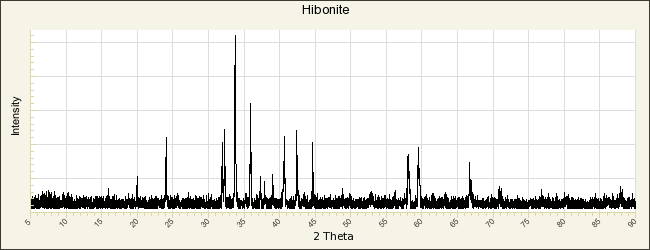
\includegraphics[width=\textwidth]{img/xrd/powder__2857__1486.png}
    \caption*{An example XRD pattern for the mineral \href{https://rruff.info/R061069}{Hibonite}.}
\end{figure}

Solids may be described as amorphous (having no discernable long-range ordering of atoms), polycrystalline (having long-range ordering, but only within small domains) or crystalline (being made up of one large crystalline domain). Generally, materials with a more ordered structure will yield XRD patterns with sharper peaks. Thus, crystalline materials will tend to yield XRD patterns with very sharp, needle-like peaks, polycrystalline materials will tend to yield XRD patterns with somewhat broader, mountain-like peaks and amorphous materials will tend to yield XRD patterns with very broad, hill-like peaks.

\begin{figure}[h!tbp]
    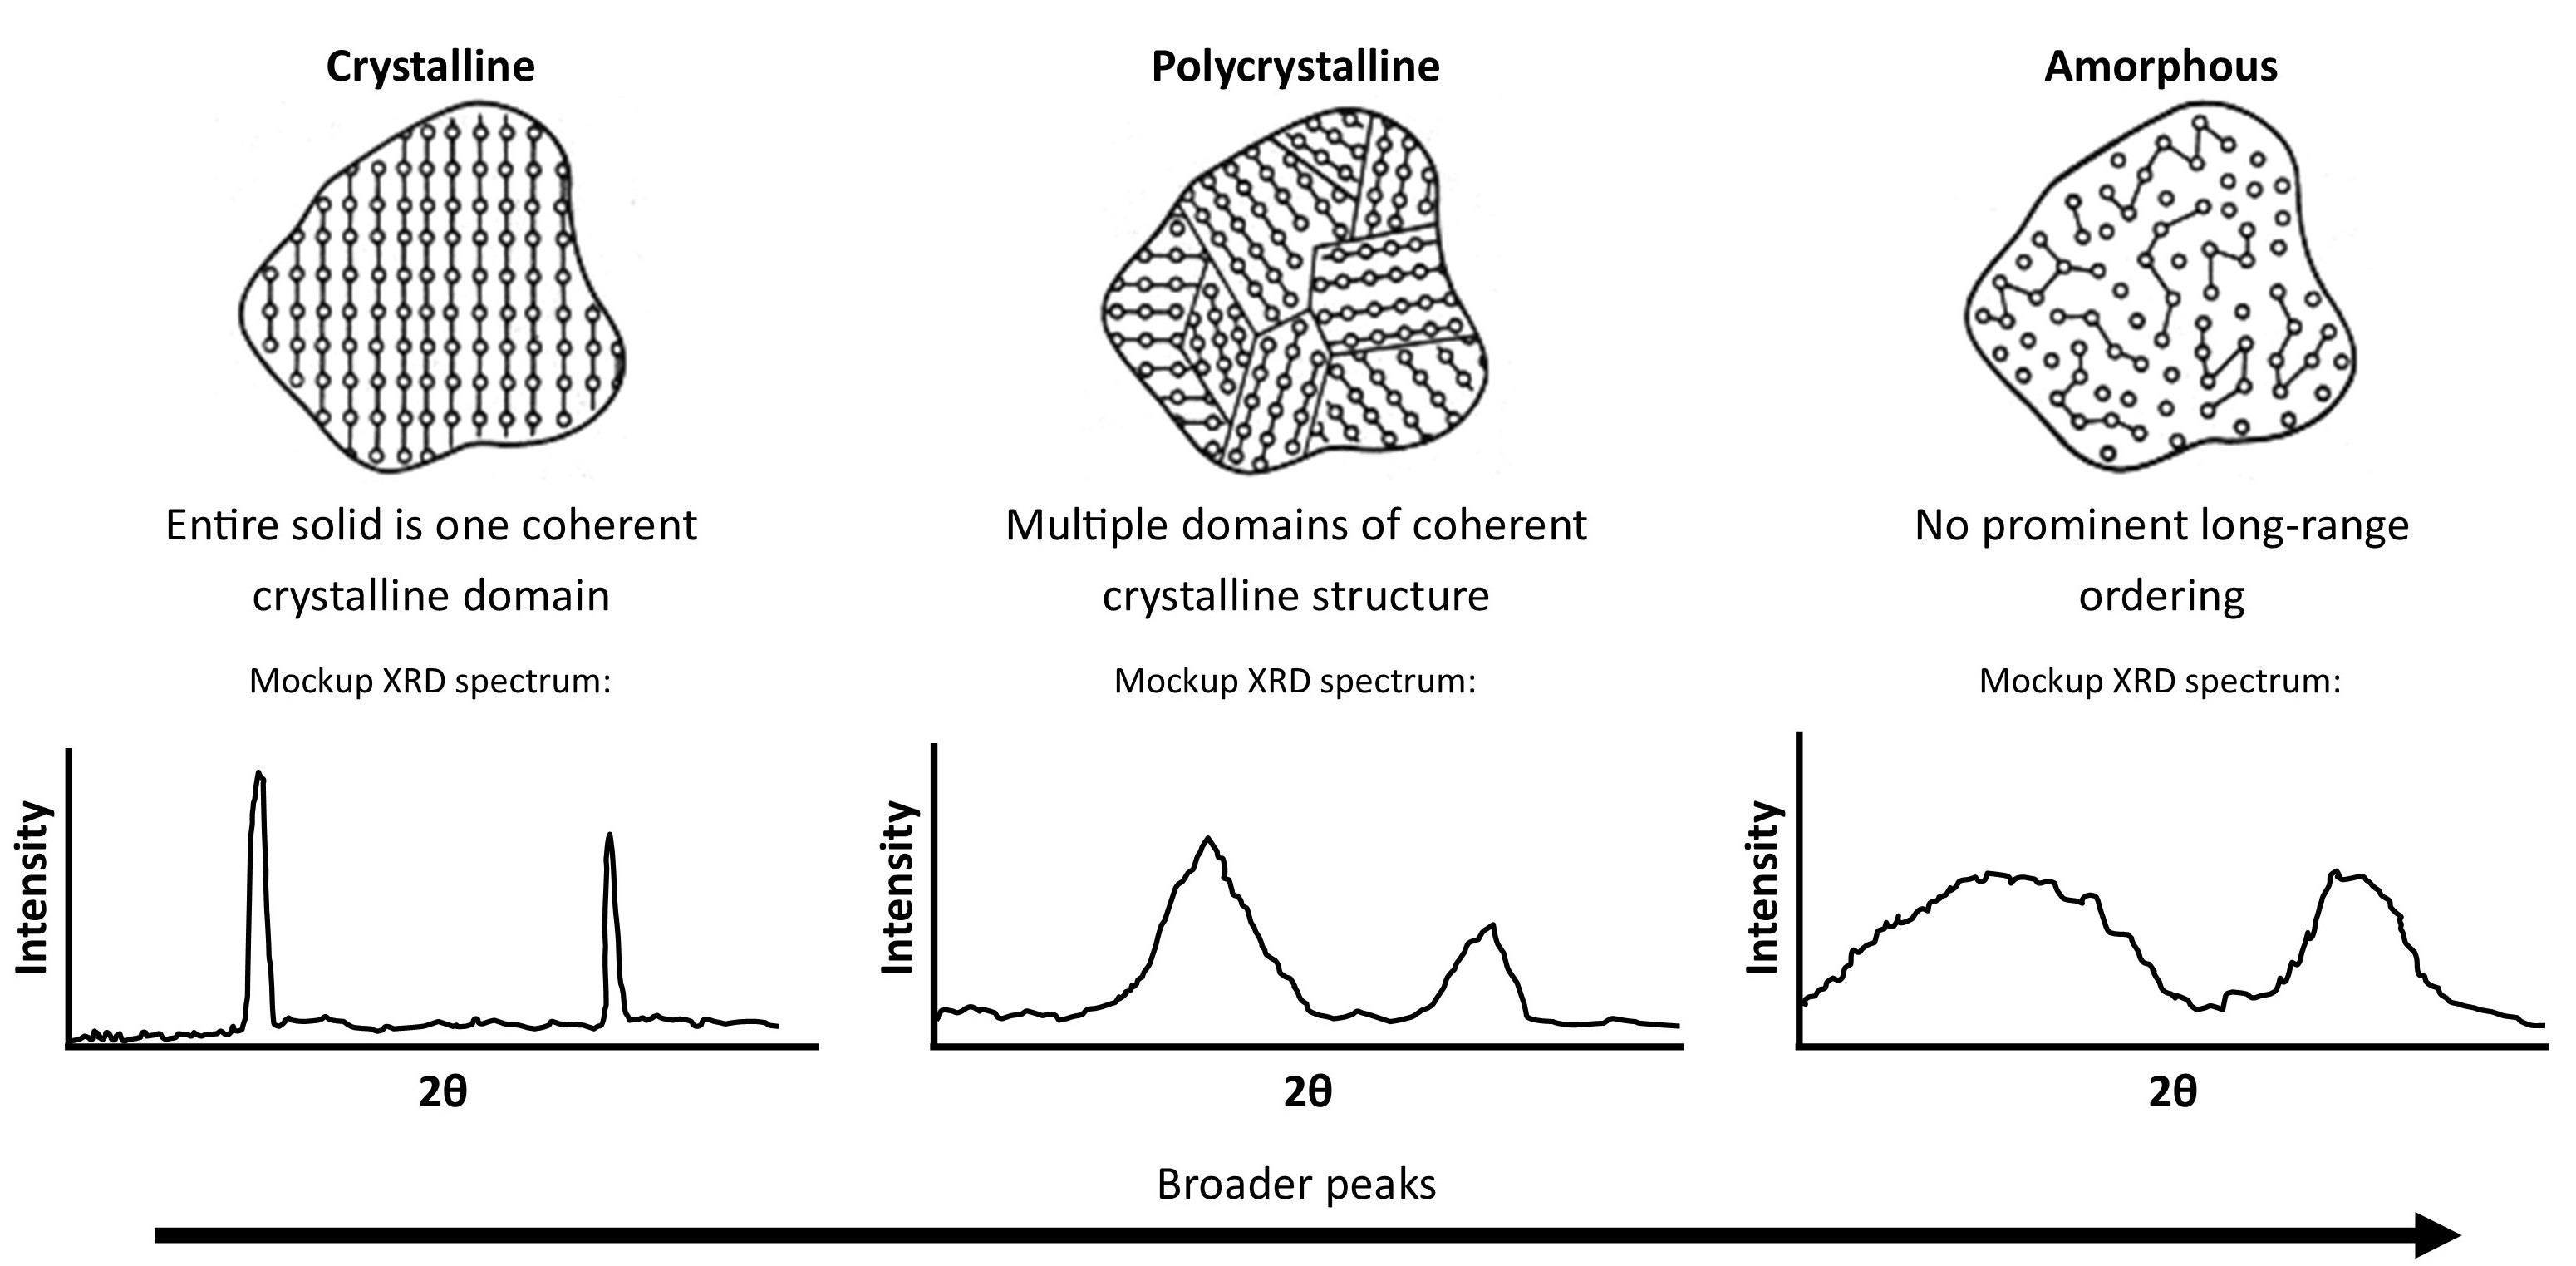
\includegraphics[width=\textwidth]{img/xrd/xrd_mockup.jpg}
    \caption*{ Materials with large crystalline domains will tend have very sharp peaks, whereas a material with no crystalline domains will tend to have very broad peaks. Note that these XRD patterns are hand-drawn to demonstrate peak broadening and do not correspond to any real material. Images adapted from \href{https://alan.ece.gatech.edu/ECE3040/Lectures/Lecture1-ElectronicMaterialsPierretChap1and2.pdf}{lecture notes of Dr. Alan Doolittle.}}
\end{figure}

\subsection*{Crystallites, grains and particles}

\href{https://www.eng.uc.edu/~beaucag/Classes/Properties%20of%20Materials/MITCrystalSizeAnalysis.pdf}{Crystallite size} describes the typical size of crystalline domains that scatter X-rays coherently (i.e., regions of the solid where the crystal lattice is all oriented the same way). \href{https://doi.org/10.1088/0957-4484/21/14/145701}{Grain size} has a similar definition, also referring to the typical size of regions of the solid where the crystal is oriented in the same direction. However, grain size is usually estimated from \href{https://en.wikipedia.org/wiki/High-resolution_transmission_electron_microscopy}{high resolution transmission electron microscopy} images and crystallite size is usually estimated from XRD patterns. A grain can be made up of a single crystallite or multiple crystallites. `Grain' and `crystallite' are often used interchangeably.

$$ \text{crystallite size} \leq \text{grain size} \leq \text{particle size}$$

\subsection*{Scherrer's equation}

\href{}{Scherrer's equation} (sometimes called the Scherrer relation or the Debye-Scherrer equation, though \href{https://doi.org/10.1038/nnano.2011.145}{not without controversy}) is a formula for estimating the mean crystallite size within a material based on the width of peaks in its XRD pattern. For a mean crystallite size of $D$, Scherrer's equation is

$$ D = \frac{K \lambda}{\beta \cos \theta} $$

where $K$ is a dimensionless shape factor (usually taken as 0.89, 0.94 or 1.0, \href{https://doi.org/10.1107/S0021889878012844}{depending on the shape of the crystal}), $\lambda$ is the wavelength of the X-rays used (usually 1.5406 \r{A}), $\beta$ is the \href{https://en.wikipedia.org/wiki/Full_width_at_half_maximum}{full width at half-maximum} of the peak in being used (in radians) and $\theta$ is the Bragg angle (in radians). Usually $D$ is estimated using only the tallest peak in the pattern. Full width at half maximum (FWHM) describes the width of the peak at the point halfway between the bottom of the peak and the top of the peak and is usually measured by fitting peaks with a Gaussian curve in software.

For assessing the integrity of crystallite size estimates made in an article using Scherrer's equation, there are three important details to note:

\begin{enumerate}
    \setlength\itemsep{-0.5em}
    \item $D$ is inversely proportional to $\beta$. In other words, as peaks become wider, crystallite sizes decrease; as peaks become narrower, crystallite sizes increase.
    \item Scherrer's equation is used for estimating crystallite size, \textit{not} particle size.
    \item Crystallite size must always be smaller than or equal to particle size.
\end{enumerate}

\subsection*{Example 1: No detectable integrity issues concerning Scherrer's equation}

In \href{https://10.0.4.64/2043-6254/ab52f7}{Mustapha et al. (2019)}, the authors use Scherrer's equation to estimate crystallite size of ZnO nanoparticles synthesized at varying pH. The XRD patterns shown in Figure 2 are consistent with the the calculated crystallite sizes shown in Table 1. Observe that as peaks become wider from pattern (a) to pattern (e), crystallite size decreases. There is nothing unexpected here. 

\begin{figure}[h!tbp]
    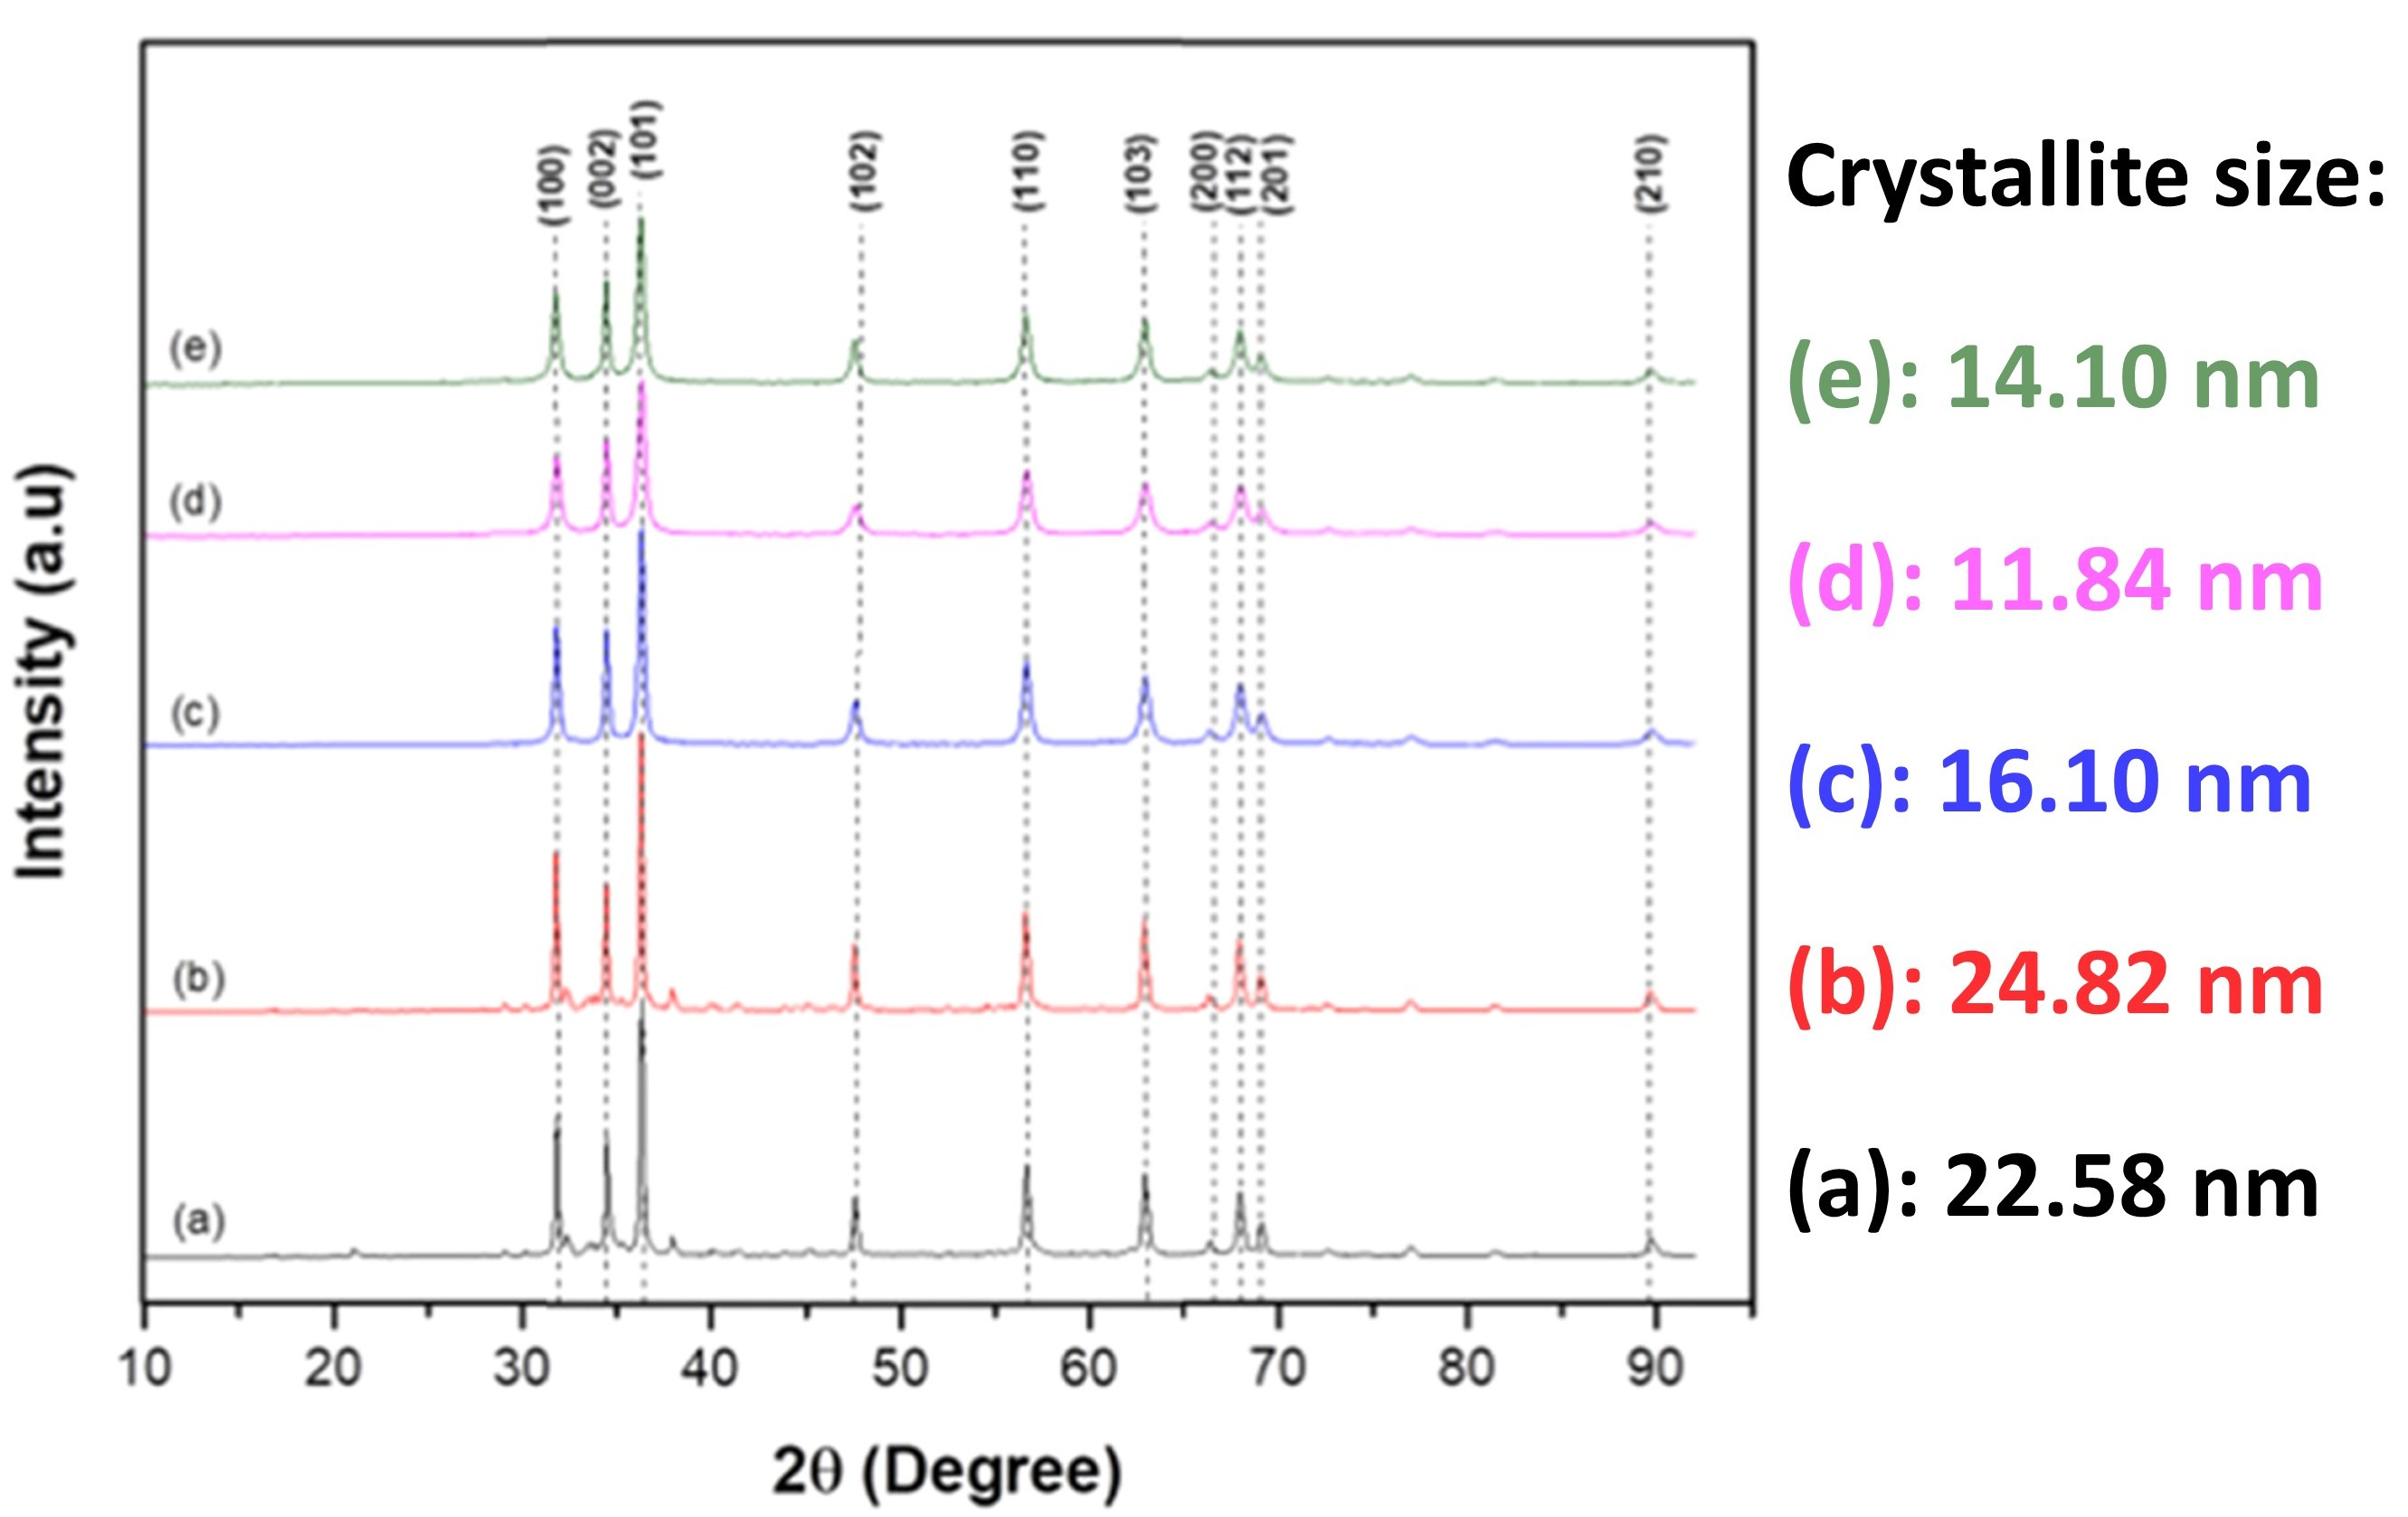
\includegraphics[width=\textwidth]{img/xrd/xrd_publication_mockup_mustapha.jpg}
    \caption*{Adapted from Figure 1 and Table 1 of \href{https://10.0.4.64/2043-6254/ab52f7}{Mustapha et al. (2019)}.}
\end{figure}

\subsection*{Example 2: Unexpected results from Scherrer's equation, inconsistency between particle sizes and crystallite sizes}

In \href{https://doi.org/10.3390/nano9071024}{Khan et al. (2019)}, the authors use Scherrer's equation to estimate crystallite sizes for Ni- and Zn-based nanoferrites. The authors state:

\begin{quote}
    \textit{The Scherrer formula is used to evaluate the particle size using the extreme intense peak (311). The experimental results demonstrate that precipitated particles’ size was in the range of 20–60 nm.}
\end{quote}

Recall that Scherrer's equation is used to estimate crystallite size, not particle size. Moreover, the authors' claimed crystallite sizes shown in Figure 2B and Table 1 imply that the (311) peak should be about three times as wide for X = 0 than X = 1. However, in Figure 2A, no such peak broadening is present in the XRD patterns shown. If anything, the (311) peak is wider for X = 1 than X = 0. 

\begin{figure}[h!tbp]
    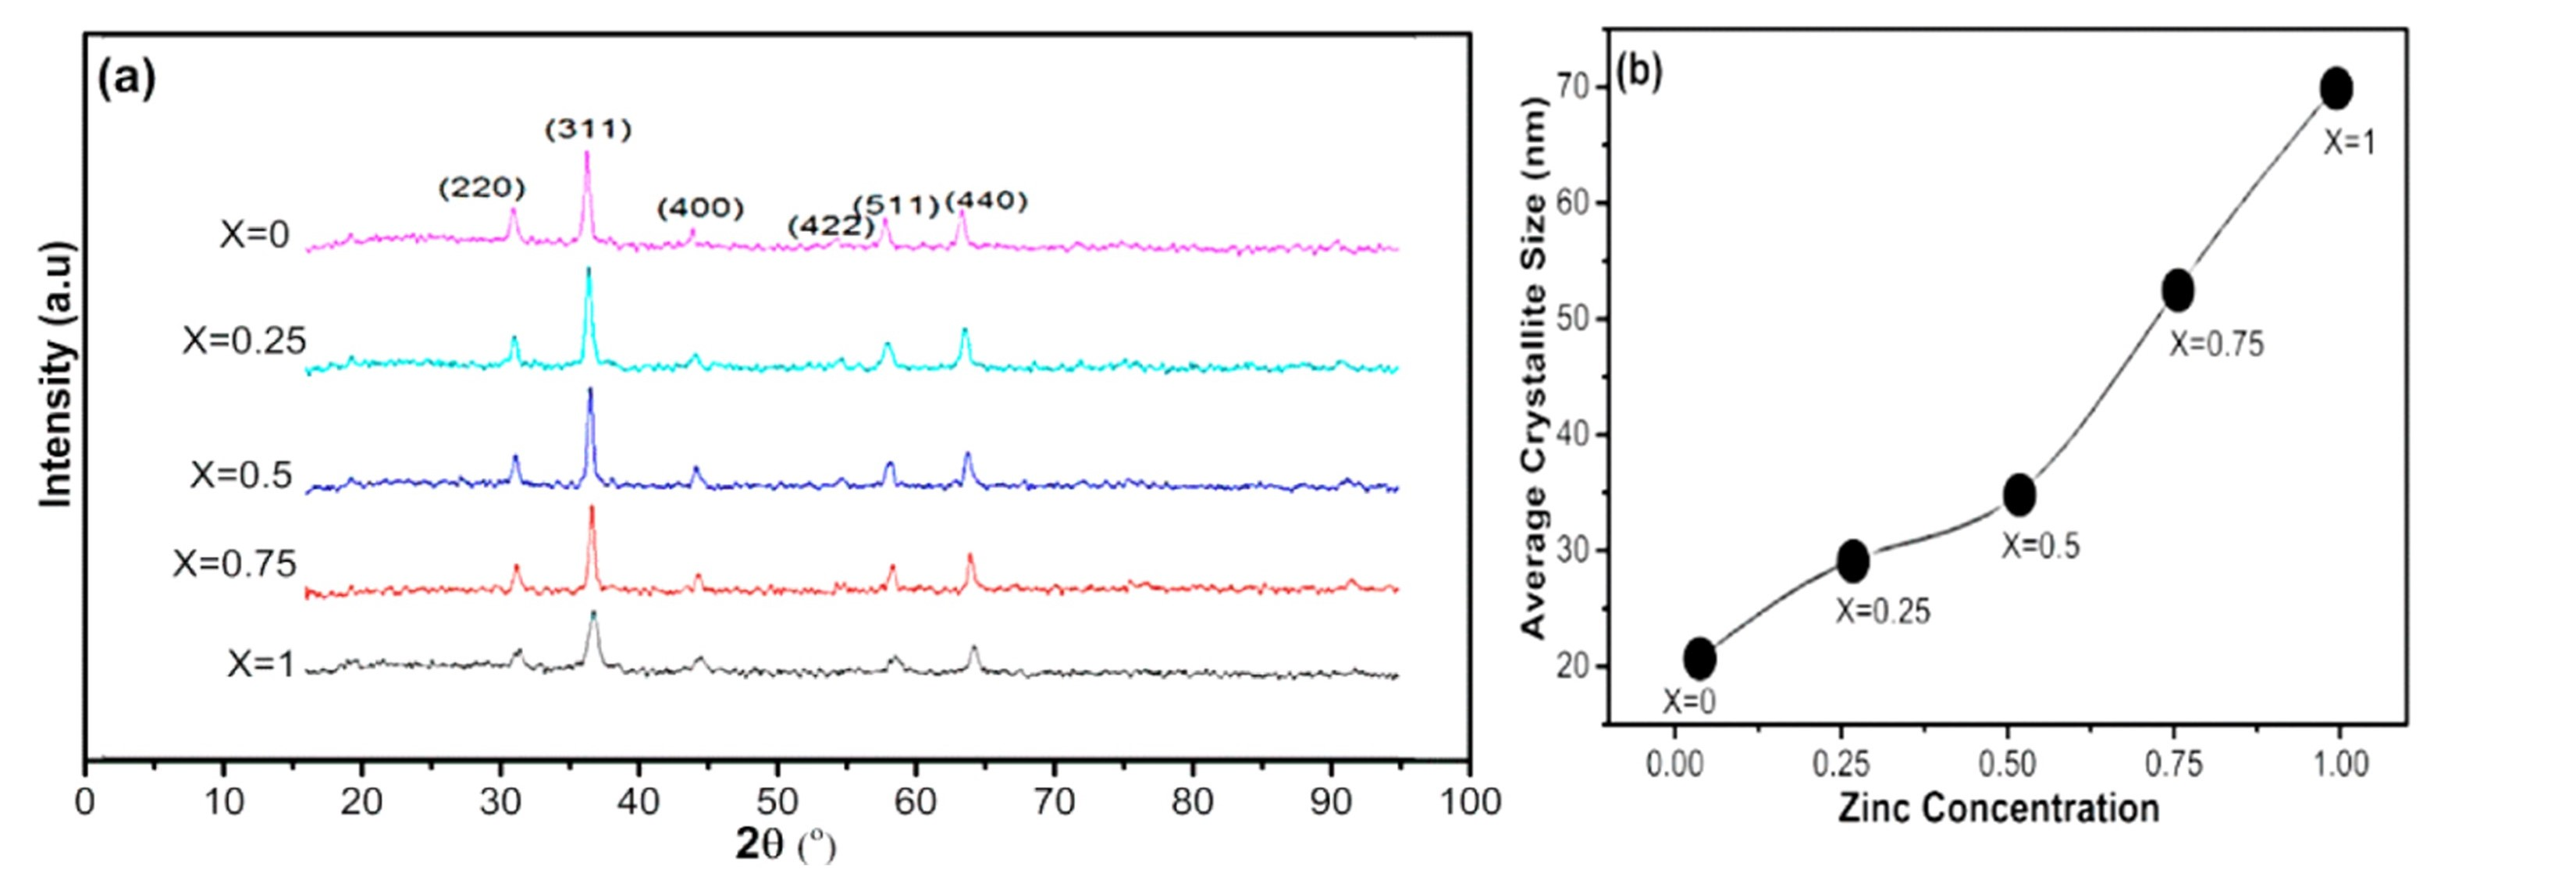
\includegraphics[width=0.8\textwidth]{img/xrd/xrd_publication_mockup_khan.jpg}
    \caption*{ Adapted from Figure 2A and Figure 2B of \href{https://doi.org/10.3390/nano9071024}{Khan et al. (2019)}.}
\end{figure}

Finally, some of the claimed crystallite sizes are larger than the nanoparticles shown for the same materials in the SEM images in Figure 1. 

\begin{figure}[h!tbp]
\centering
    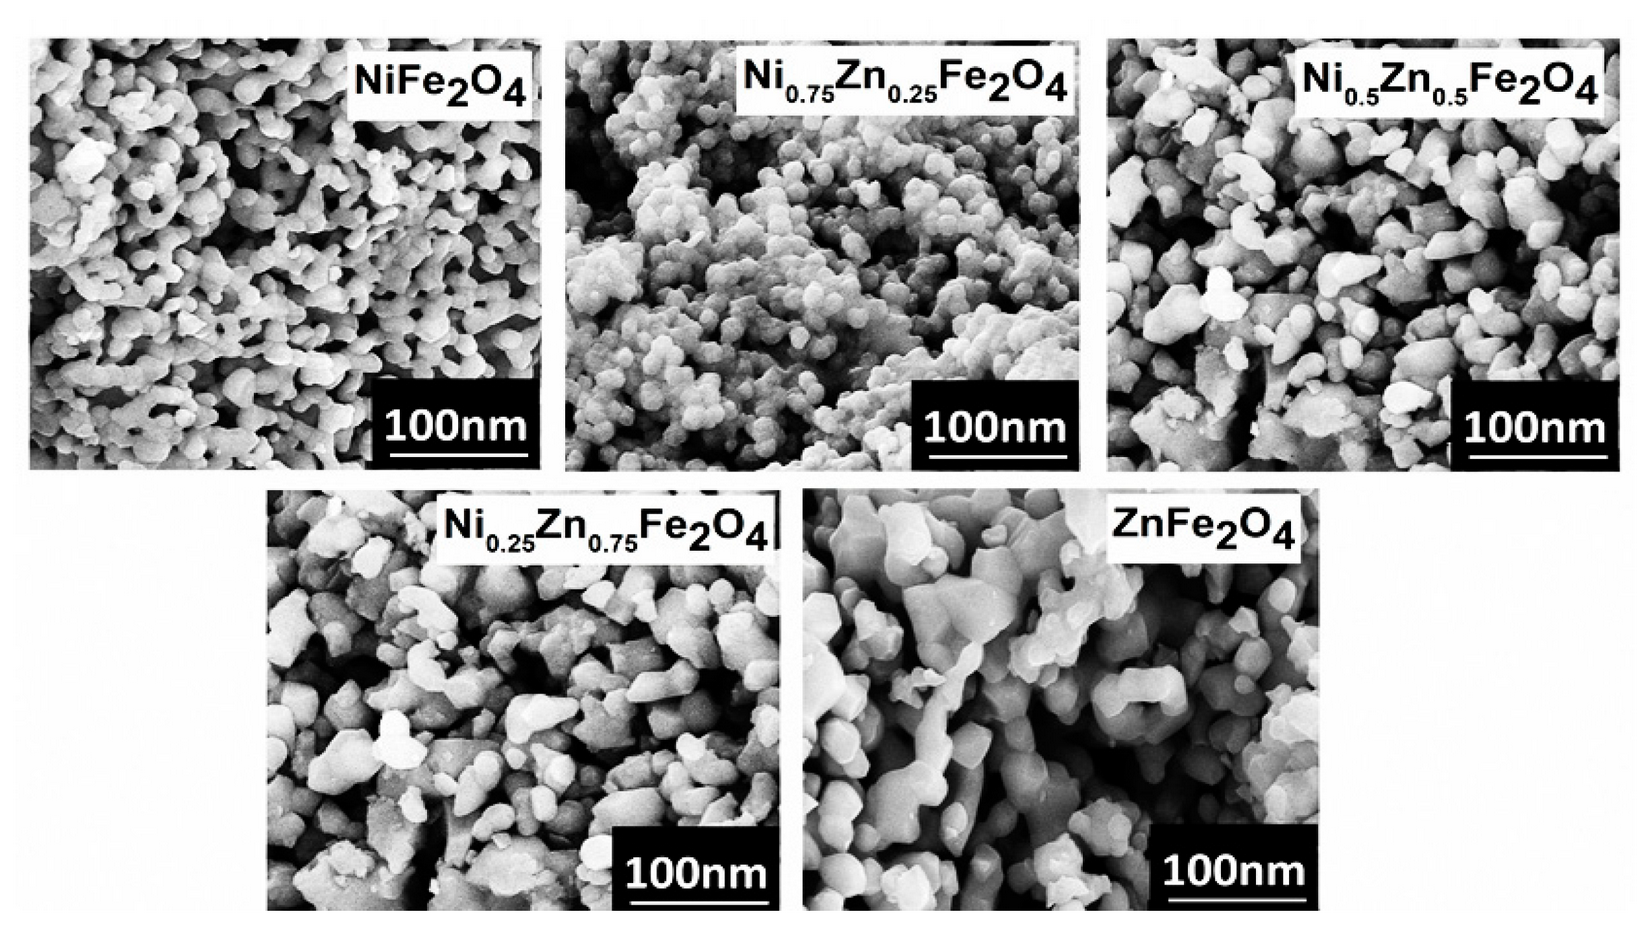
\includegraphics[width=0.8\textwidth]{img/xrd/xrd_sem_images_khan.jpg}
    \caption*{ Adapted from Figure 1 of \href{https://doi.org/10.3390/nano9071024}{Khan et al. (2019)}.}
\end{figure}

\subsection*{Example 3: Unexpected results from Scherrer's equation}

In \href{https://doi.org/10.1021/acs.energyfuels.2c03279}{Abdullah et al. (2023)}, the authors use Scherrer's equation to estimate crystallite sizes of AgTe nanostructures. They state:

\begin{quote}
    \textit{Effect of Ag0.006Te, Ag0.012Te, Ag0.025Te, Ag0.05Te, and Ag0.1Te nanostructure was determined with crystallite size found in the range of 85 nm, 73 nm and 39 nm, and 67 nm and 88 nm, respectively, measured with Debye Scherer.}
\end{quote}

If the crystallite size of Ag0.025Te is twice as small as its counterparts, one would expect the peaks in the XRD pattern for Ag0.025Te to be twice as wide. However, this is not observed in the XRD patterns shown in Figure 1A. In fact, the patterns shown for all materials in Figure 1A are identical except for vertical scaling.

\begin{figure}[h!tbp]
\centering
    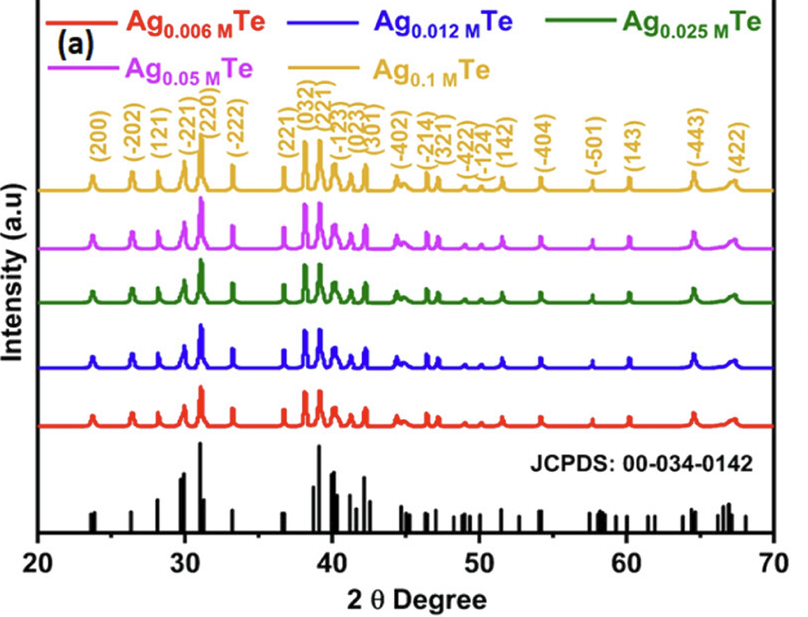
\includegraphics[width=0.7\textwidth]{img/xrd/xrd_spectra_abdullah.png}
    \caption*{ Adapted from Figure 1A of \href{https://doi.org/10.1021/acs.energyfuels.2c03279}{Abdullah et al. (2023)}.}
\end{figure}

\subsection*{Example 4: confusion of crystallite size with particle size}

In \href{https://doi.org/10.1016/j.jallcom.2016.03.279}{Upadhyay et al. (2016)}, the authors use Scherrer's equation to estimate crystallite sizes of magnetite nanoparticles. However, throughout the article the authors refer to crystallite size and particle size interchangeably, several times claiming that particle size can be determined by Scherrer's equation. For instace, the caption of Table 1 reads:

\begin{quote}
    \textit{Table 1. Particle size, lattice parameter and strain in the sample calculated from X-ray data. Size (S) represent particle/crystallite size calculated using Scherer formula while Size (WH) represent particle/crystallite size calculated from Williamson–Hall method.}
\end{quote}

\end{document}